%%%%%%%%%%%%%%%%%%%%%%%%%%%%%%%%%%%%%%%%%%%%%%
\section{Beamline}
\label{sec:h4beamline}

The H4 beamline is extended to the NP04 cryostat in the newly constructed extension of EHN1. To produce particles in the momentum range of interest, 80 GeV/c pion beam from the the T2 primary target is impinged on a secondart Cu target to generate a tertiary beam. The tertiary particles are momentum and charged-selected and transported down the H4 beamline to the experimental area. The H4 beamline can operate in parallel with the H2 beamline minimize interference between the two ProtoDUNE experiments.

\subsection{H4 Beamline layout and optics}

A sketch of the H4 beamline layout is shown in Figure~\ref{fig:H4layout}. The first two dipole magnets (shown in red) after the secondary target are rotated by about 56$^\circ$ to move the beam downward towards the cryostat. The third dipole magnet (shown in green) is for sweeping the beam into one of the three beam windows.
\begin{cdrfigure}[H4 beamline layout]{H4layout}{Sketch of the H4 beamline layout in the region near the cryostat (Courtesy of V. Clerc, CERN).}
  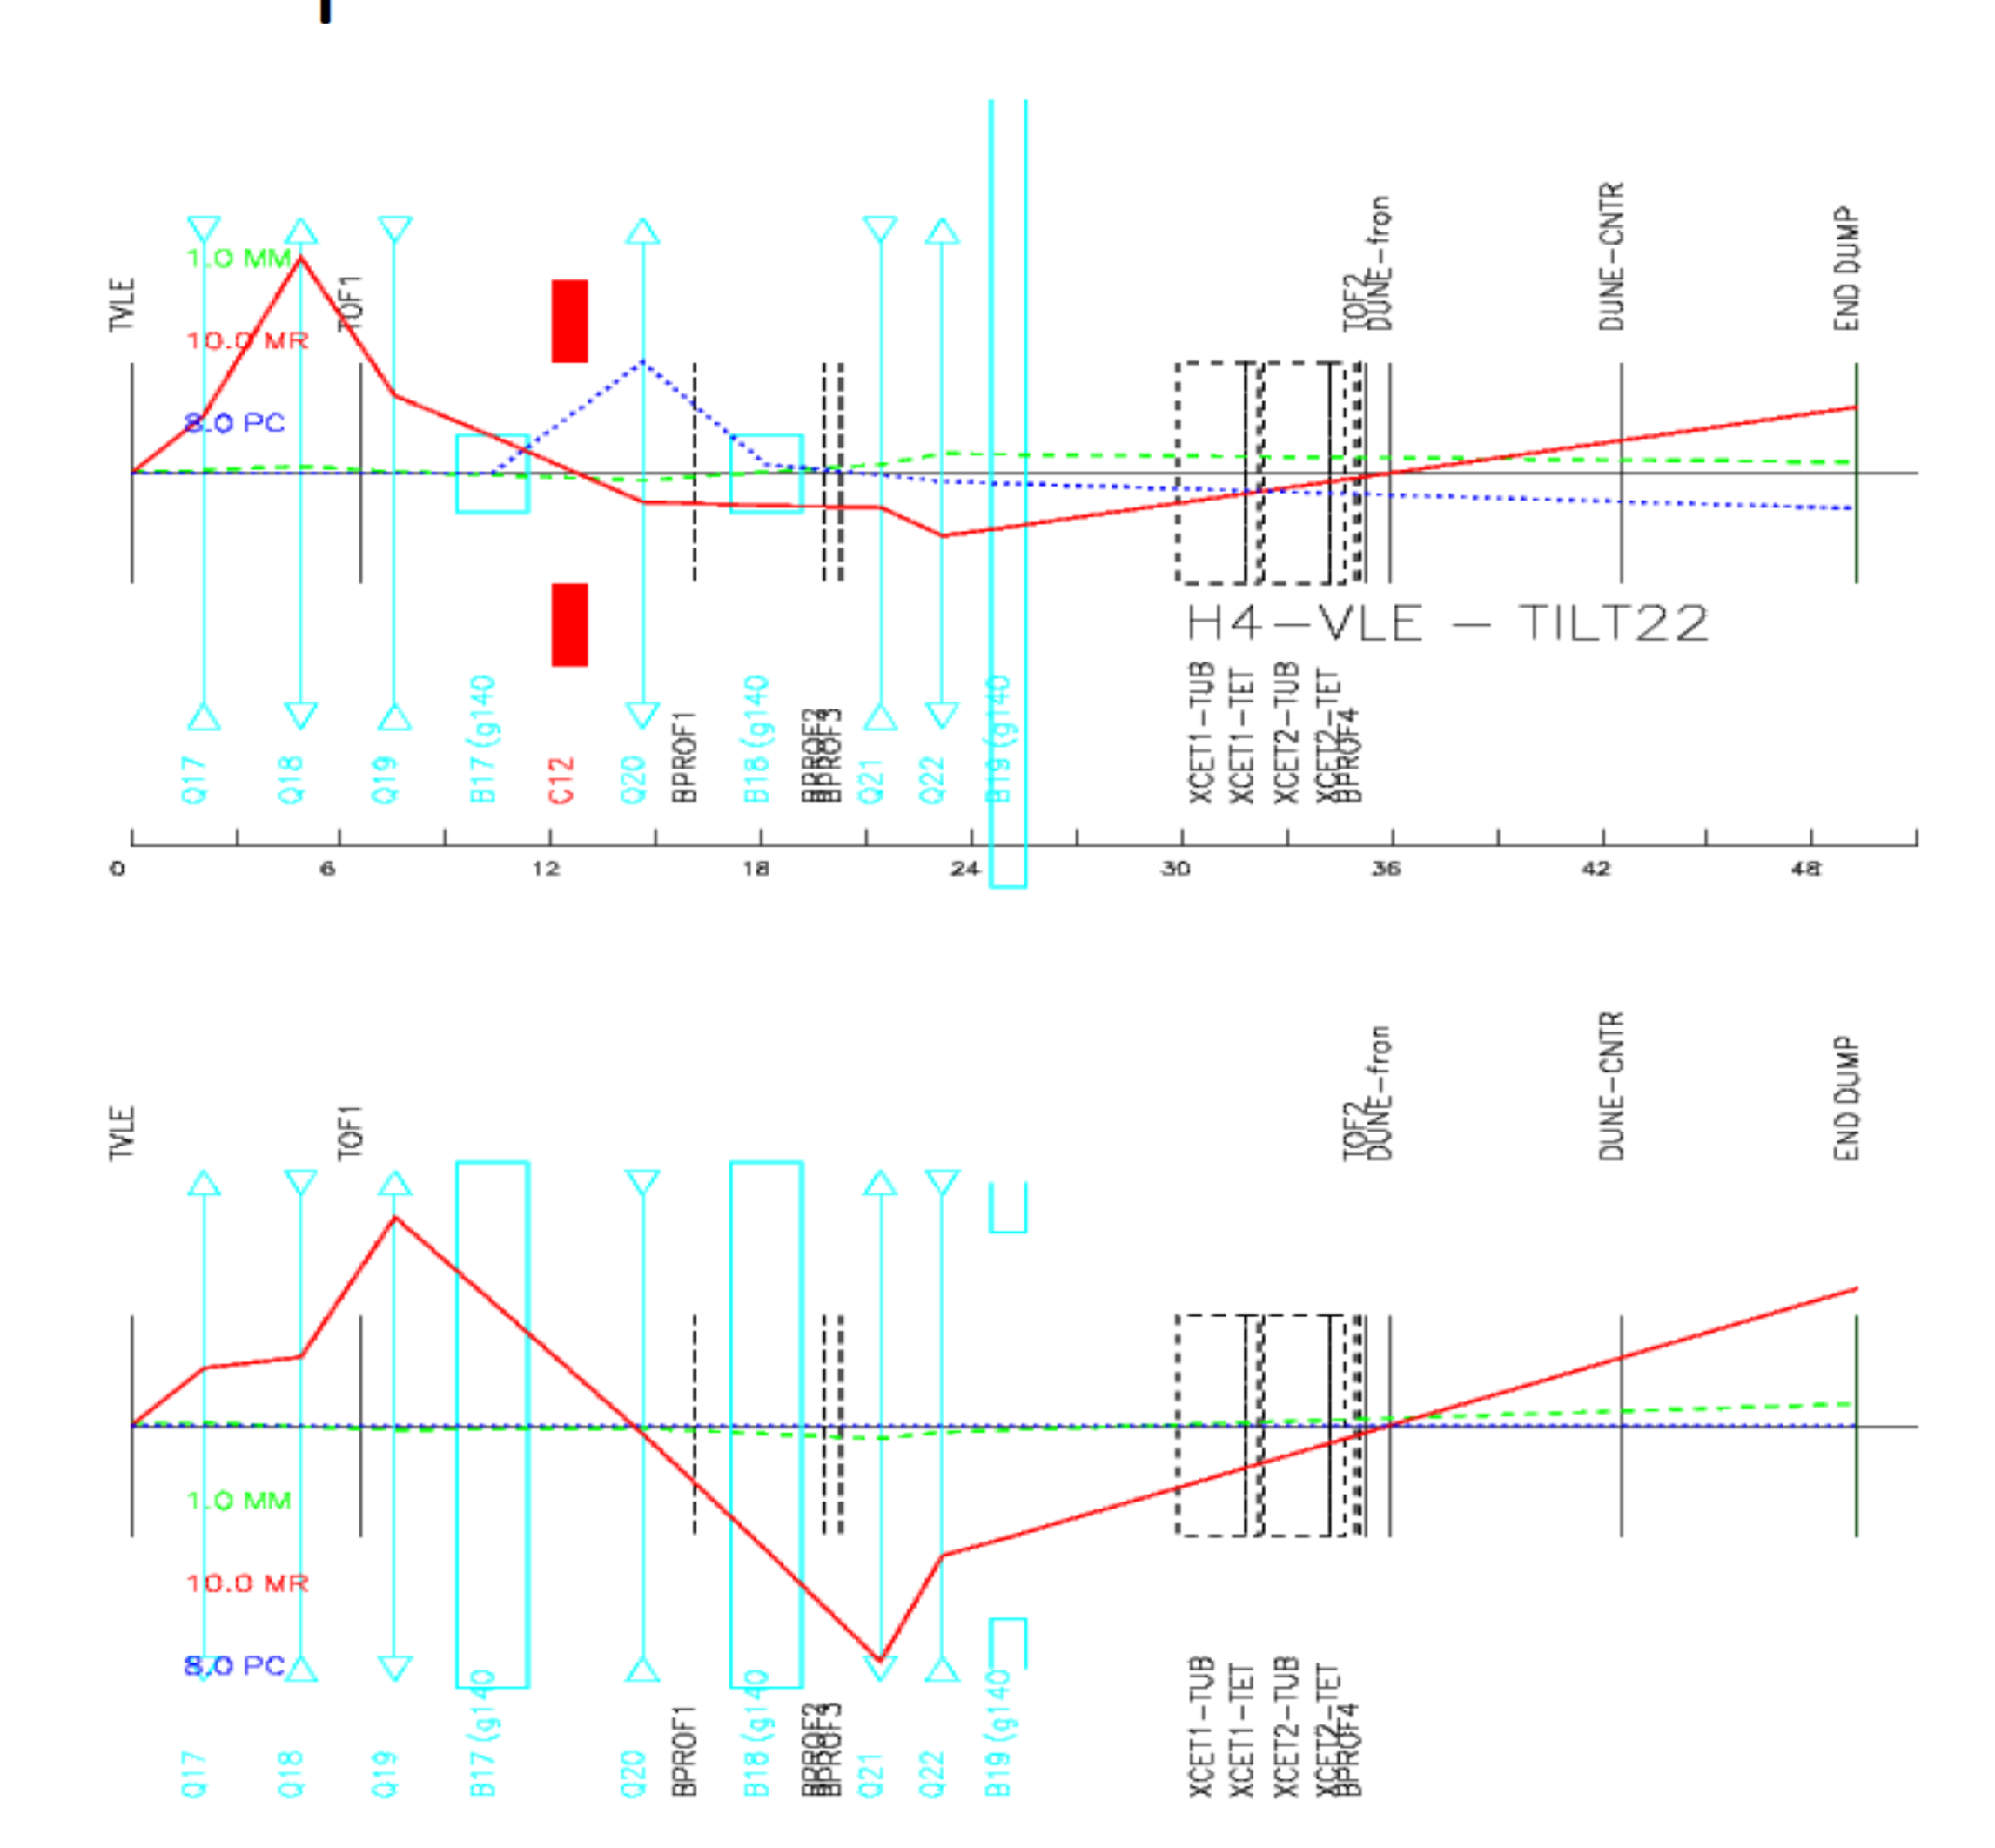
\includegraphics[width=0.95\textwidth]{beamline_H4layout.pdf}
\end{cdrfigure}


The beamline optics for the horizontal and vertical planes are shown in Figure~\ref{fig:beamoptics}. The series of dipole and quadropole magnets focus and direct the beam to one of the three beam windows. For this particular configuation, the beam is focused at the front of the cryostat.
\begin{cdrfigure}[H4 beam optics]{beamoptics}{H4 beamline optics for the horizontal (top) and vertical (bottom) planes. The secondary target is located on the left side of the plots and the front of the ProtoDUNE-SP cryostat is located at the beam focus point, at about 33m from the secondary target.}
  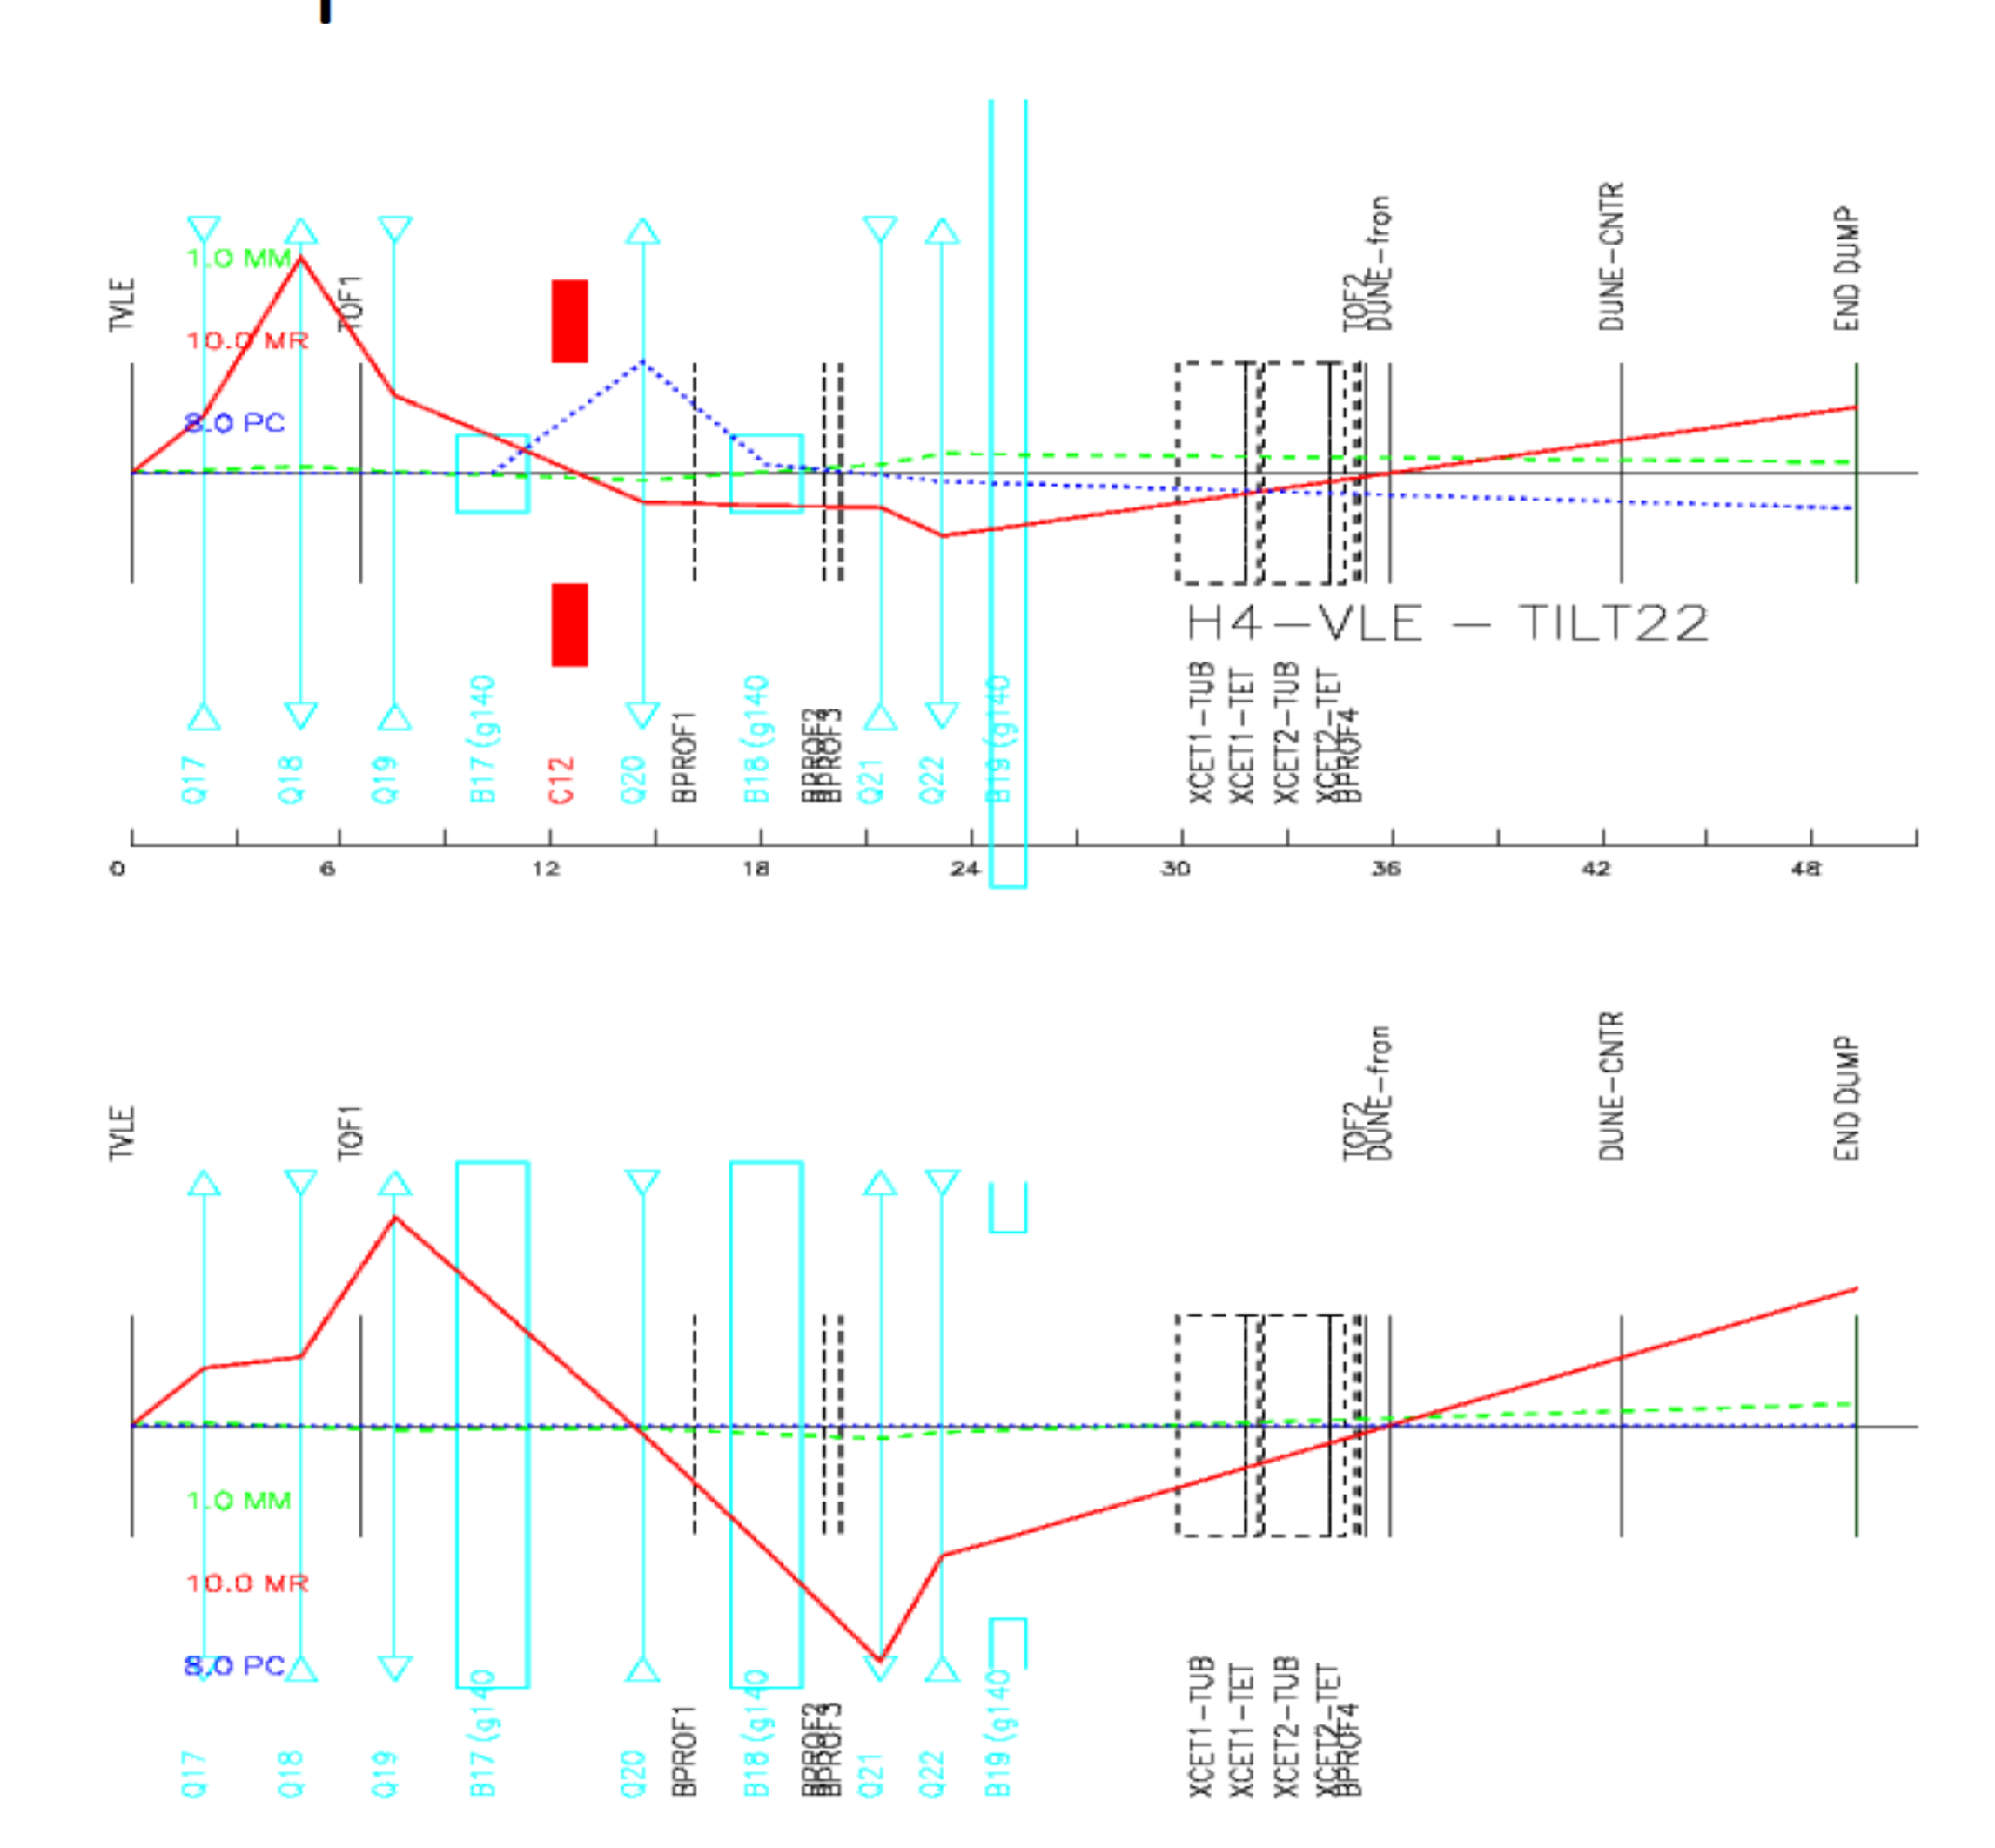
\includegraphics[width=0.99\textwidth, angle=-90]{beamline_H4Optics.pdf}
\end{cdrfigure}

\subsection{Beam properties}
\fixme{Need simulation results from Nikos}
A full simulation of the H4 beamline has been recently performed (courtesy of N. Charitonidis). Preliminary results are included in the following (a full check of the results has to be performed).
The GEANT4 model includes the H4 upstream beamline and the tertiary
beamline.  Target, magnets, collimators and a preliminary assumption
about beam instrumentation are included. The secondary target has been
modeled as a R=30mm L=300mm Tungsten cylinder for   E$<3$GeV and a s a Copper cylinder of the same dimensions  if E$>=$3 GeV. Optimization of the target is ongoing.

Table \ref{tab:beampartcomp} describes the particle composition of the
beam at the entrance of the cryostat. Two features are evident. The
former  is that the beam is dominated by positrons at low energies,
the latter  is that the kaon content, and in a lesser extent the pion
one, are  depleted by decays along the beam path. 

\begin{cdrtable}[Beam composition]{cccccc}{beampartcomp}{Beam composition (in percentage)  at the cyostat entrance, particles contained in the beam pipe.}
Momentum (GeV/c) & e$^+$ & $K^+$ & $\mu^+$ & p& $\pi^+$ \\ \toprowrule
1 & 69.7 & 0& 0.3 & 17.3 & 12.7\\ \colhline
2 &37.2& 0.6& 1.7& 24.1&36.3\\ \colhline
3 & 63.6&0.8&0.6&8.2&26.8\\ \colhline
4 & 46.4 & 1.8 & 1.1 & 8.5 & 42.1 \\ \colhline
37.2 & 2.8 & 0.9 & 8.6 & 50.6\\ \colhline
27.7 & 4.0 & 0.9& 10.2 & 57.3\\ \colhline
20.7 & 4.8 & 1.0 & 10.7 & 62.8 \\
\end{cdrtable}
%%%%%%%%%%%%%%%%%%%%%%
Achievable particle rates, assuming a spill intensity of $10^6$
particles on the secondary target and the SPS spill length of 4.8
seconds are reported in Table~\ref{tab:beampartrates}. 
\begin{cdrtable}[Trigger rate]{ccccccc}{beampartrates}{Trigger rates.}
Momentum (GeV/c) & e$^+$ & $K^+$ & $\mu^+$ & p& $\pi^+$& total\\ \toprowrule
1 & 14 & 0 & 0 & 4 & 3  & 20 \\ \colhline
2 & 10 & 0 & 0 & 7 & 10 & 27 \\ \colhline
3 & 90 & 1 & 1 & 12 & 38 & 141\\ \colhline
4 & 68 & 3 & 2 & 12 & 61 & 146\\ \colhline
5 & 56 & 4 & 1 & 13 & 76 & 149\\ \colhline
6 & 47 & 7 & 1 & 17 & 97 & 169\\ \colhline
7 & 41 & 9 & 2 & 21 & 123& 196\\
\end{cdrtable}

At momenta larger than about 4 GeV/c, the particle rates are near to the
maximum acceptable rate to avoid event pileup, that is around
100Hz.  At lower energies, the proton and pion rate is much lower, down
of  factor of 10 at 1 or 2 GeV/c, and is, as already said, overwhelmed
by the positron rate.

The momentum spread of the beam is of the order of 5 to 7 \%. At higher energies, where
the particle rate is higher, the momentum spread  can be narrowed by
closing the collimators, at the expenses of the beam intensity.  For example, Figure \ref{fig:momcoll} shows
that at p=4~GeV/c the momentum uncertainty can be  reduced to $\Delta p/p= 3.6\%$ with a factor 4 reduction in trigger rate.  
\begin{cdrfigure}[Beam momentum uncertainty]{momcoll}{Beam momentum uncertainty with different collimator openings at 4 GeV/c.}
  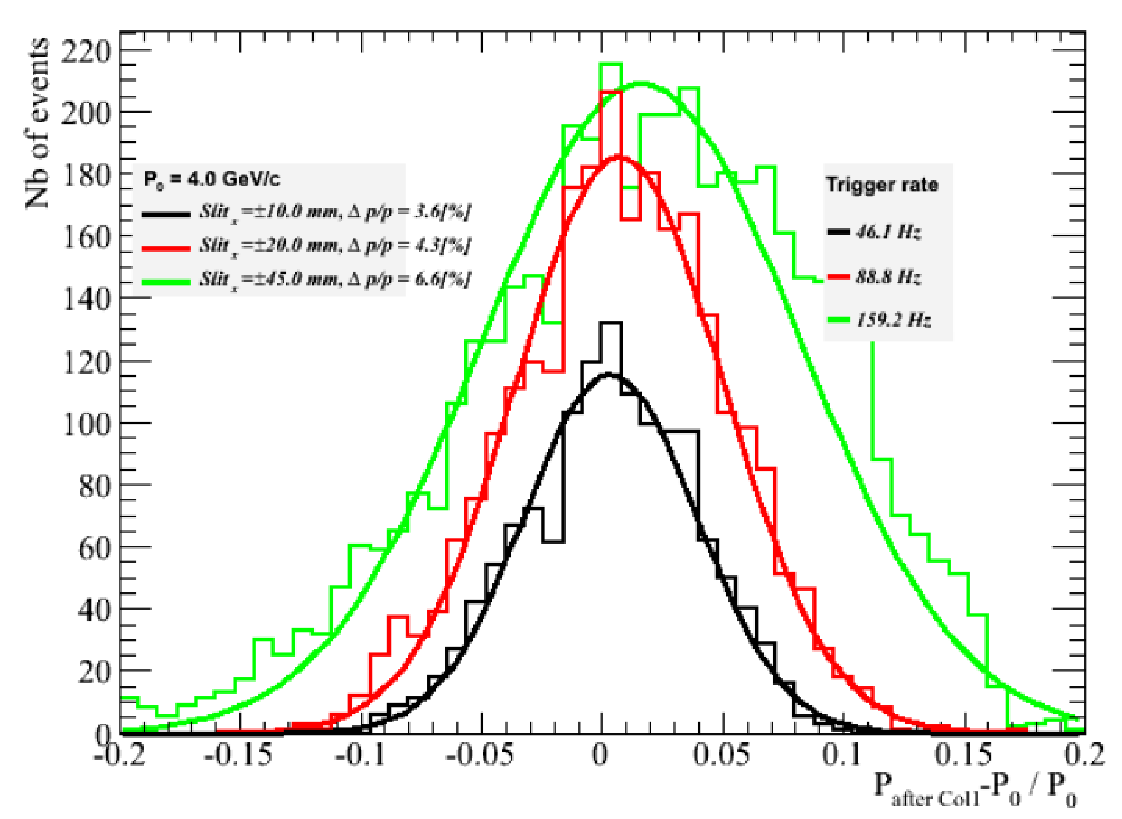
\includegraphics[width=0.95\textwidth]{Slits.pdf}
\end{cdrfigure}

\subsection{Muon halo}
The secondary beam at 80 GeV is mainly composed by pions. In the long path  between the primary and the secondary target, an intense high energy muon halo is produced by pion decay. Muons propagate approximately in the direction of the H4 beamline, that is slightly pointing upwards, therefore the most intense part of the muon halo passes above the ProtoDUNE SP cryostat. 
Figure \ref{fig:muonhalo_HE} shows the spatial distribution of the muon halo at the cryostat face. Only muons with momentum larger than 4~GeV/c have been consuidered. Despite the (still) low statistics, the upwards asymmetry is clearly visible. The axis origin is set approximately at the centre of the cryostat face. The color scale gives the muon intensity in $\mu /m^2/spill$ for $10^6$ particles/spill from the primary target. Muon intensity on the cryostat ranges from  from $\approx 1$ to $\approx 500 $ $\mu /m^2/spill$.
This plot is very preliminary, not only because of low statistics: shielding around the low energy beam line is not included in the simulation, and the muons produced in the other beamlines in H1N1, including the H2 line that feeds the DualPhase ProtoDUNE, are not considered here. 
\begin{cdrfigure}[Muon halo intensity at the cryostat face]{muonhalo_HE}{Muon halo intensity at the cryostat face. The axis are centerd on the cryostat, dimensions are in mm. Color scale  in $\mu /m^2/spill$, with a lower threshold at $P_\mu = 4$~Gev/c.}
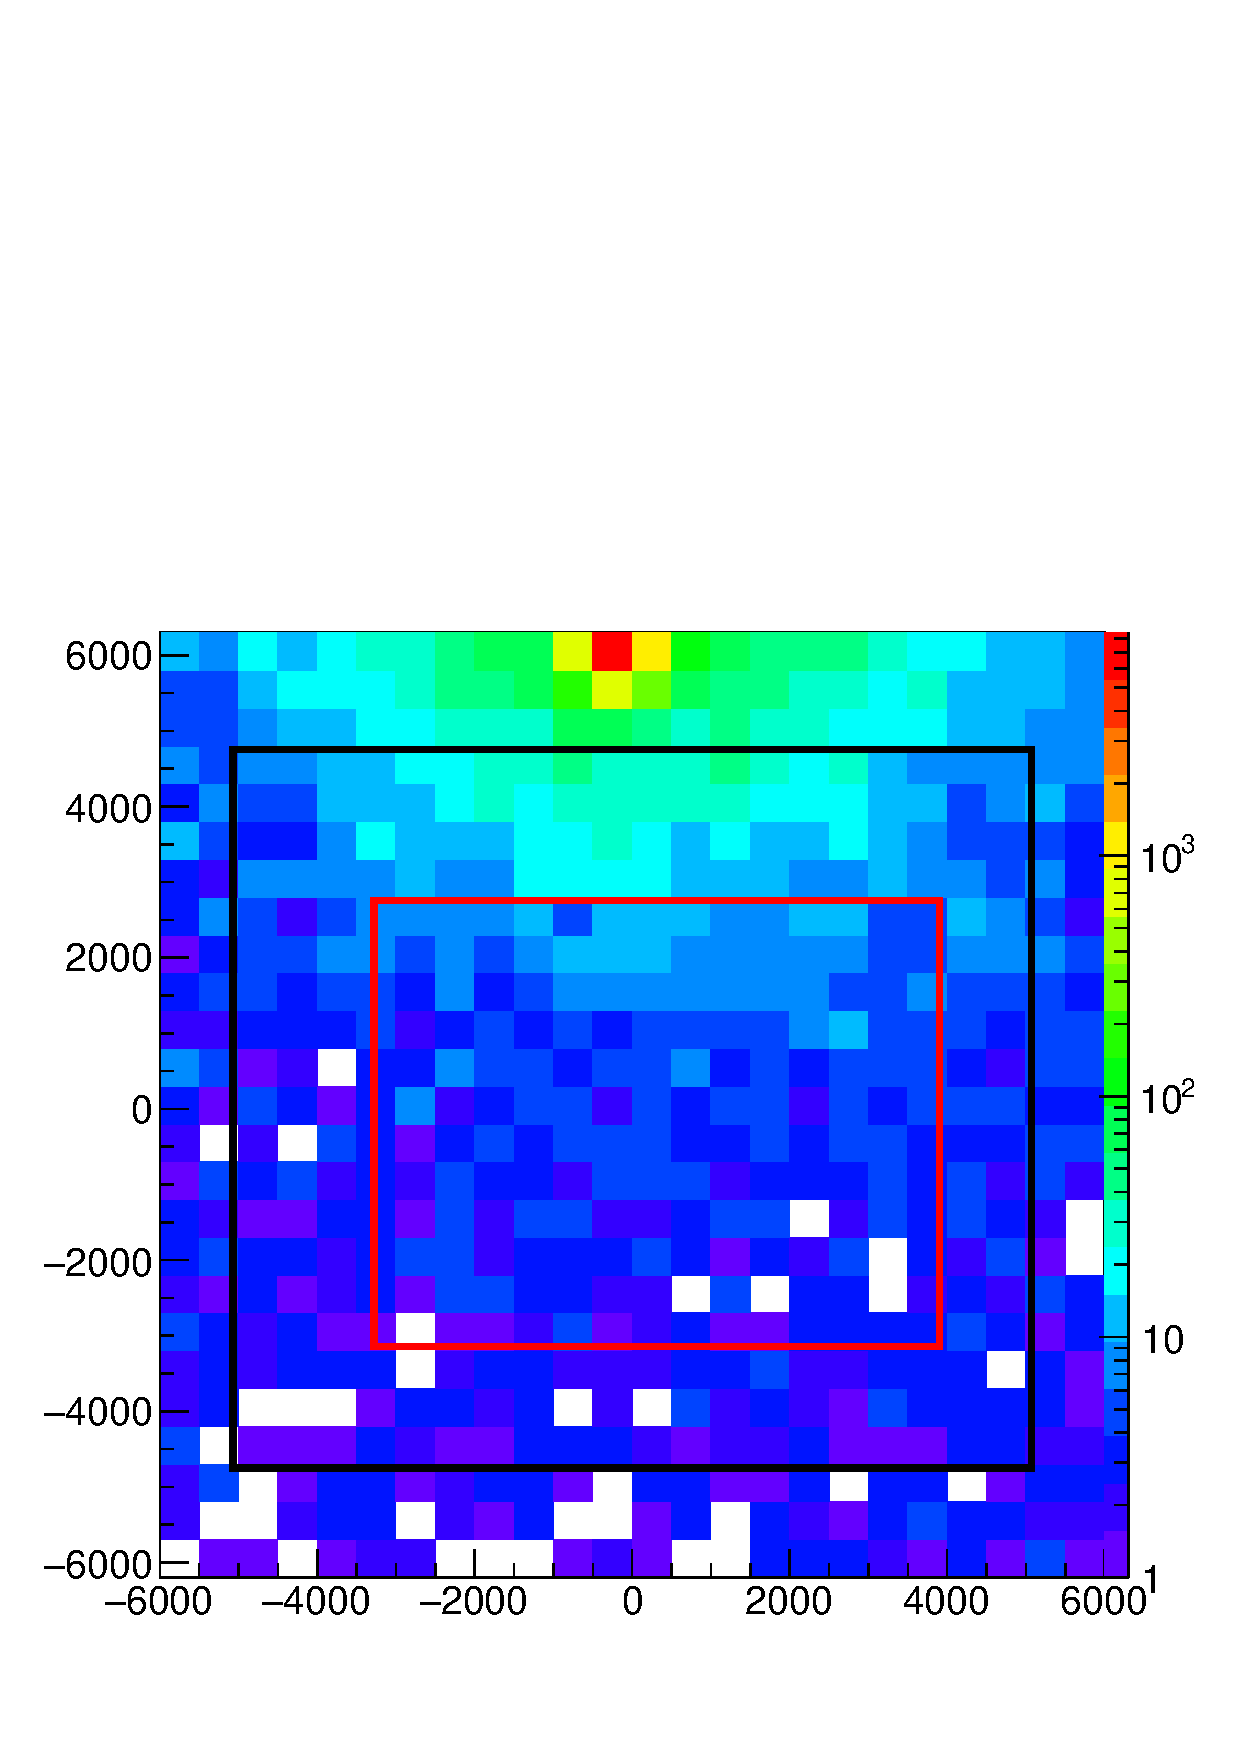
\includegraphics[width=0.95\textwidth]{muon_map_HE_square.pdf}
\end{cdrfigure}





